%!TEX TS-program = xelatex
%!TEX encoding = UTF-8 Unicode
\documentclass[12pt,twoside,a4paper]{memoir}
\usepackage{fontspec,xltxtra,xunicode}
\usepackage{polyglossia}
	\setmainlanguage{italian}
    \PolyglossiaSetup{italian}{indentfirst=false} % rientra anche il primo capoverso dopo il titolo di sezione
	
\defaultfontfeatures{Mapping=tex-text}
\setromanfont[Mapping=tex-text]{TeX Gyre Termes} % va da 12pt
%\setromanfont[Mapping=tex-text]{TeX Gyre Pagella} % basta 11pt
%\setromanfont[Mapping=tex-text]{TeX Gyre Schola} 
%\setromanfont[Mapping=tex-text]{TeX Gyre Bonum} 
\setsansfont[Scale=MatchLowercase,Mapping=tex-text]{TeX Gyre Adventor}
%\setsansfont[Scale=MatchLowercase,Mapping=tex-text]{TeX Gyre Heros}
%\setsansfont[Scale=MatchLowercase,Mapping=tex-text]{Futura}
\setmonofont[Scale=MatchLowercase]{Andale Mono}
%
% *********************PACCHETTI******************
\usepackage{metalogo,lipsum}
\usepackage[colorinlistoftodos,italian,textsize=footnotesize,prependcaption]{todonotes}
\usepackage{paralist}
\usepackage{enumitem}
\usepackage[italian]{varioref}  	%pantieri p. 40 
\usepackage{comment}
\usepackage[output-decimal-marker={,}]{siunitx} % virgola nei decimali
\usepackage{color,soul}
\usepackage{graphicx}
%-----------------------------------
% figure
\usepackage[labelfont={normalsize,bf},font={small,sf}]{caption} % modifico la didascalia delle figure
%***********************************
% CROSS-REFERENCES -- P295 MEMman
% ***********************************
\renewcommand{\tref}[1]{Tabella \vref{#1}} % ridefinisco \tref (di memoir) per tradurlo in italiano e dirgli di comportarsi come \vref o \ref
\renewcommand{\fref}[1]{Figura \vref{#1}}
\renewcommand{\Aref}[1]{Appendice \ref{#1}} 
\renewcommand{\Cref}[1]{Capitolo \vref{#1}} 
\renewcommand{\Sref}[1]{Sezione \vref{#1}} 
\renewcommand{\Pref}[1]{Parte \ref{#1}} 
% 
\usepackage{textcomp} % per i gradi
\usepackage{siunitx}
%-----------------------------------
%----------------ULTIMO PACCHETTO---
%-----------------------------------
\usepackage{xcolor}
\definecolor{burgundy}{rgb}{0.5, 0.0, 0.13}
\usepackage{hyperref}% mi serve che ci sia
\hypersetup{%
colorlinks=true,% se = false circonda il testo del link 
linkcolor=burgundy,% comanda anche l'indice
%urlbordercolor=1 0 0 
urlcolor=red,%
citecolor=green, % colora {in verde} i link attivi
pdfauthor={arch. Federico Morchio},%
pdfsubject={regolamento edilizio},%
pdfkeywords={26_11, regolamento edilizio, allegato energetico-ambientale},%
}%
% *************************************
%\setlength{\parindent}{0em} % no indentazione in memoir
% *************************************
%*-----------------------------COPERTINA
% *************************************
%----------------------------------
\newcommand*{\plogo}{\fbox{$\mathcal{OA}$}} % logo PROVVISORIO 
% -----------------------------------
% COPERTINA - FRONTESPIZIO - TITLE PAGE --
% -----------------------------------
\newcommand*{\titleGM}{\begingroup % Create the command for including the title page in the document
\hbox{ % Horizontal box
\hspace*{0.2\textwidth} % Whitespace to the left of the title page
\rule{1pt}{\textheight} % Vertical line
\hspace*{0.05\textwidth} % Whitespace between the vertical line and title page text
\parbox[b]{0.75\textwidth}{ % Paragraph box which restricts text to less than the width of the page
{\noindent\huge\bfseries Comune di Casal Cermelli \\[0.5\baselineskip] \Large{Provincia di Alessandria \\ Regione Piemonte}}\\[5\baselineskip] % Title
{\Large\textbf{Regolamento Edilizio Comunale}}\\[2\baselineskip] % Tagline or further description
{\fbox{\Large \textsc{\textcolor{blue}{Allegato Energetico Ambientale }}}} \\[3\baselineskip] % Tagline or further description+ colore by fede
{\Large \textsc{Regolamento Edilizio Comunale}} \\ 

\textit{Progettista:} \\ arch. Federico Morchio % Author name
\medskip\\   \raggedright

{\hspace{13em}\rlap{\raisebox{-1.30\baselineskip}[0pt][0pt]{\includegraphics[angle=0]{timbro-ordine.pdf}}}\\
}
%\textit{Collaboratori:} \\ arch. Andrea Gamondo 
\medskip

{15076 Ovada (AL) -  via Gramsci 109 \\ progettazione@oikosatelier.it - (39) 0143.80233 \par} % Editor affiliation

\vspace{0.08\textheight} % Whitespace between the title block and the publisher
Il resp. del procedimento: geom. Vilmo G. Bovone\\

\vspace{0.12\textheight} % Whitespace between the title block and the publisher

{\noindent oikosatelier \plogo}\date: Ottobre 2016\\[\baselineskip] % Publisher and logo
}}
\endgroup% 
}
%---------------------------
% FINE COPERTINA
% --------------------------
%------------------------------------
% TOC Style
%------------------------------------
\setcounter{tocdepth}{0} % 0 numera PART+Chapter
%\setcounter{secnumdepth}{3}
%\setsecnumdepth{subsection} % va inserito se voglio numerate anche le subsections
%\setsecnumdepth{subsubsection}
\addto\captionsitalian{\renewcommand{\partname}{TITOLO}}  
%\addto\captionsitalian{\renewcommand{\chaptername}{Articolo}}  % 
\renewcommand\cftpartname{\partname~} % "part NAME" nel TOC
\renewcommand\cftchaptername{\chaptername~} % "CHAPTER NAME" nel TOC
%
\setlength{\cftpartnumwidth}{3em} % nel TOC allarga la colonna
%
% **************************************************
% --------INCLUDE--ONLY--PREAMBLE----------------------
% --------------------------------------------------
\includeonly{% non commentare qua ma nel DOCUMENT
% FRONTMATTER%
0-frontmatter/0-premessa,% no estensione.tex
%<percorso file>,%
%***********************************
% MAINMATTER
%===================================
1-mainmatter/introduzione,%
1-mainmatter/geometria-solare,%
% APPENDIX
%
% BACKMATTER
3-backmatter/colophon,%
}% chiude tutto
%
%
% *********************************************
% -----------------------INIZIO DOCUMENTO
% *********************************************
\begin{document}
%
\frenchspacing % OBBLIGATORIO vedi guida guitt beccari
\tightlists % solo in memoir per restingere spazi nelle liste
%\firmlists 
\pagestyle{empty}  	% COPERTINA --- Removes page numbers
 % per non avere header e footer
\titleGM % copertina tipo mia
% -----------------------------
% STILI DI PAGINA ALTERNATIVI 
% ----------------------------- 
%\chapterstyle{madsen}   	% BEI NUMERONI!
\chapterstyle{lyhne}   		% usalo in caso di titoli lunghi.
%\chapterstyle{ell}  		% occhio ha solo il numero senza Articolo o Capitolo
%\chapterstyle{tandh}% 
% ********************************
% -----------------------FRONTMATTER
% ********************************
%
\frontmatter
% !TEX root = ../26_11c-all-en-amb-master-ok.tex

\chapter{Premessa}
\label{chp:premessa}

\section{Principali norme di riferimento}
\label{sec:norme-riferimento-princ}

Il presente documento è redatto ai sensi delle vigenti normative nazionali e piemontesi.


\section{Nota concettuale}
\label{sec:nota-import}

L'allegato Energetico Ambientale ad un Regolamento Edilizio –~a nostro avviso~– deve riportare essenzialmente \emph{i principi di base che regolano la progettazione e la realizzazione} di interventi su edifici – nuovi o esistenti – con attenzione verso gli aspetti della \emph{sostenibilità}, della \emph{bioclimatica}, della \emph{bioarchitettura} e del \emph{benessere complessivo} per i fruitori dei manufatti  – che nella maggioranza dei casi coincidono con i committenti – e delle persone che dall'esterno vivono l'ambiente in cui tali manufatti sono inseriti.

La proposta, alternativa, di un estratto di normative ed un elenco di dati – concepiti come limiti prestazionali e/o descrizione tecnica di sistemi tecnologici – originerebbe importanza marginale e transitoria, poste la variabilità delle disposizioni di legge in materia energetica a cui abbiamo assistito negli ultimi anni e la rapida e costante mutazione prestazionale delle tecnologie connesse al mondo dell'edilizia. È probabile che, in questo modo, l'allegato nascerebbe già vecchio. 

La proposizione di regole – perlopiù fondate sul \emph{buonsenso progettuale} e sul \emph{rispetto di pochi ma fondamentali principi guida} – appare una via più efficace,  fermo restante che questo allegato costituirà una base di riferimento che il Comune potrà implementare  nel tempo senza incorrere in stravolgimenti operativi fastidiosi per i progettisti, per i committenti e per coloro che dovranno verificare le effettive rispondenze delle loro proposte edificatorie al presente regolamento.




 % no estensione .tex
% *************************************
% INSERISCO QUA GLI INDICI
% *************************************
\renewcommand*\contentsname{Indice del documento} %modifica il nome all'indice
% \textcolor{purple}{\listoftodos} %list of todo colorata ELENCO COSE DA FARE
%va disabilitato nella versione finale
\clearpage
\tableofcontents*  % Nb l'asterisco in 'memoir' evita che nell'indice venga scritto anche 'indice' con la relativa pagina.
\clearpage
\listoffigures*    % idem come x TOC
\newpage
\listoftables*    % idem come x TOC
\newpage
% bozza del ----- preso dal collaudo 55_1
%
% ho mescolato 3 scenari prefigurati da madsen in 'Page styles on steroids or memoir makes page styling easy"
\addtopsmarks{headings}{% fede:scenario n.1 di Madsen
\nouppercaseheads % added at the beginning
}{%
  \createmark{subsection}   {right}{shownumber}{}{. \space}
  \createmark{subsubsection}{right}{shownumber}{}{. \space}
}
% use the new settings
\newcommand\AddRevision{%  scenario n.6 che sarebbe per le revisioni ma posso usare per scrivere anche altro.
\setlength\unitlength{1mm}
   \begin{picture}(0,0)
   \put(0,-7){\footnotesize\itshape\textcolor{purple}{bozza del \today}}
 \end{picture}}
 \makeoddfoot{headings} {\AddRevision}{}{}
 \makeevenfoot{headings}{\AddRevision}{}{}
 \makeoddfoot{plain}    {\AddRevision}{\thepage}{}
 \makeevenfoot{plain}   {\AddRevision}{\thepage}{}
\pagestyle{headings} 
\makeheadrule{headings}{\textwidth}{\normalrulethickness}%scenario n.7 linea sotto header
%\pagestyle{headings}
%%%%%%%%%%%%%%%%%%%%%%%%
% ********************************
% -----------------------MAINMATTER
% ********************************
\mainmatter
% !TEX root = ../26_11c-all-en-amb-master-ok.tex

\chapter[Introduzione]{INTRODUZIONE ALL'ALLEGATO ENERGETICO AMBIENTALE}
\label{chp:allegato-en-amb}

\section{Interventi assoggettati all'allegato}
\label{sec:interventi-assogg}

\todo[inline]{vanno valutati bene sulla base delle norme}

I principi contenuti nel presente allegati sono applicabili a tutti i tipi interventi edilizi. Vanno osservati obbligatoriamente per le seguenti tipologie e per quelle ad esse assimilabili in via interpretativa o per specifica deliberazione comunale:

\begin{itemize}
\item nuova costruzione
\item ristrutturazione edilizia
\item sostituzione edilizia
\item ristrutturazione urbanistica
\item ampliamento
\item la sopraelevazione
\item il completamento che presupponga cambio di destinazione o nuovo volume
\item cambio di destinazione d'uso di locali esistenti da trasformare a scopo residenziale o per attività lavorative che presuppongano il soggiorno di persone nei nuovi locali (uffici, negozi e assimilabili)
\end{itemize}

Per gli edifici assoggettati a vincolo ai sensi del codice dei beni architettonici le norme di tutela prevalgono sugli aspetti trattati dal presente allegato.

\section{Contenuti dell'allegato:}
\label{contenutidellallegato:}

L'allegato:

\begin{itemize}
\item riporta indicazioni progettuali di massima. Il progettista le approfondirà in funzione dei propri obiettivi e delle proprie conoscenze

\item definisce alcune linee guida progettuali da seguire per migliorare i livelli prestazionali degli edifici attraverso la progettazione (bioclimatica) più attenta ai principi di sostenibilità;

\item fornisce idee che il progettista potrà sviluppare autonomamente in virtù delle proprie conoscenze, inclinazioni e attitudini;

\item definisce azioni di progettazione specificatamente mirate alla sostenibilità che possono consentire di ottenere incentivi:

\begin{itemize}
\item \emph{economici} che si traducono in risparmi sugli oneri di costruzione

\item \emph{volumetrici} che si traducono in percentuali di incremento rispetto al volume edificabile ottenibile applicando i parametri urbanistici associati alla zona territoriale urbanistica o all'edificio oggetto di intervento

\end{itemize}

\end{itemize}

\section{A cosa serve l'allegato}
\label{acosaservelallegato}

È uno strumento di supporto alla progettazione per tutti gli interventi edilizi: sia quelli assoggettati obbligatoriamente ai suoi contenuti sia gli altri per i quali assume valore di riferimento ed appoggio progettuale.

Per gli interventi elencati in \Sref{sec:interventi-assogg} il progettista ha l'obbligo di seguire le indicazioni progettuali descritte nel presente allegato che vanno considerate alla stessa maniera di quelle contenute nel regolamento edilizio che definiremo classico.

In estrema sintesi l'allegato energetico ambientale fornisce indicazioni e regole che consentono di utilizzare anche gli elementi naturali – radiazione solare, acqua, vento, luce, ombra – come potenziali sistemi di riscaldamento o raffrescamento gratuiti che vanno affiancati ai materiali ed ai sistemi impiantistico adoperati per garantire i rispetto delle norme e dei regolamenti in ambito igienico-sanitario energetico-prestazionale ed edilizio-regolamentare.

In seconda battuta la sua finalità consiste nel definire una serie di azioni progettuali e realizzative che – in virtù delle ricadute sul piano della sostenibilità che ne derivano – consentono al committente di ottenere benefici in termini di qualità abitativa ed eventuali incentivi e sgravi calcolati sulla base di specifiche tabelle commisurate al grado prestazionale aggiuntivo ottenuto a livello progettuale, a livello costruttivo e a livello operativo (nel ciclo di vita).

\section{Come si usa l'allegato}
\label{comesiusalallegato}

Va visto ed interpretato come un \emph{manuale tecnico} che fornisce una sintesi di indicazioni che il progettista ed il committente sceglieranno in relazione agli obiettivi qualitativi che si sono prefissati. 

Concettualmente va considerato come un supporto operativo per il progettista piuttosto che come un ulteriore documento normativo di appesantimento delle procedure per l'ottenimento delle necessarie autorizzazioni ai lavori.

Contiene (anche) l'indicazione di comuni errori progettuali a cui generalmente corrispondono divieti: esattamente come accade per il regolamento classico, pensiamo ad esempio al rispetto delle distanze tra gli edifici o tra pareti finestrate. In questo senso va considerato che a livello progettuale possono essere analizzati e coretti numerosi aspetti che, in caso contrario, non potrebbero essere più affrontati – con gli stessi costi e la stessa efficacia – una volta avviato il cantiere e costruito il volume. La \fref{fig:efficacia-decis-lechner} evidenzia graficamente come, all'interno di un processo edilizio, le decisioni prese nelle prime fasi – assumano  maggiore efficacia in termini controllo e riduzione dei costi di edificazione ed di impatto ambientale. Mentre man mano che la costruzione avanza, fino a percorrere ed esaurire il proprio ciclo di vita il campo delle possibilità e delle alternative si restringe significativamente. \\ Pensiamo, ad esempio, a fattori determinanti come la definizione dimensionale degli spazi e dei volumi, all'orientamento dell'edificio, alla disposizione interna relazionata all'orientamento, e riflettiamo sulle ricadute delle decisioni in ordine al risparmio energetico ed al benessere interno per gli occupanti.

\begin{figure}[htbp]
\centering  % ordine per clip: left, lower right upper
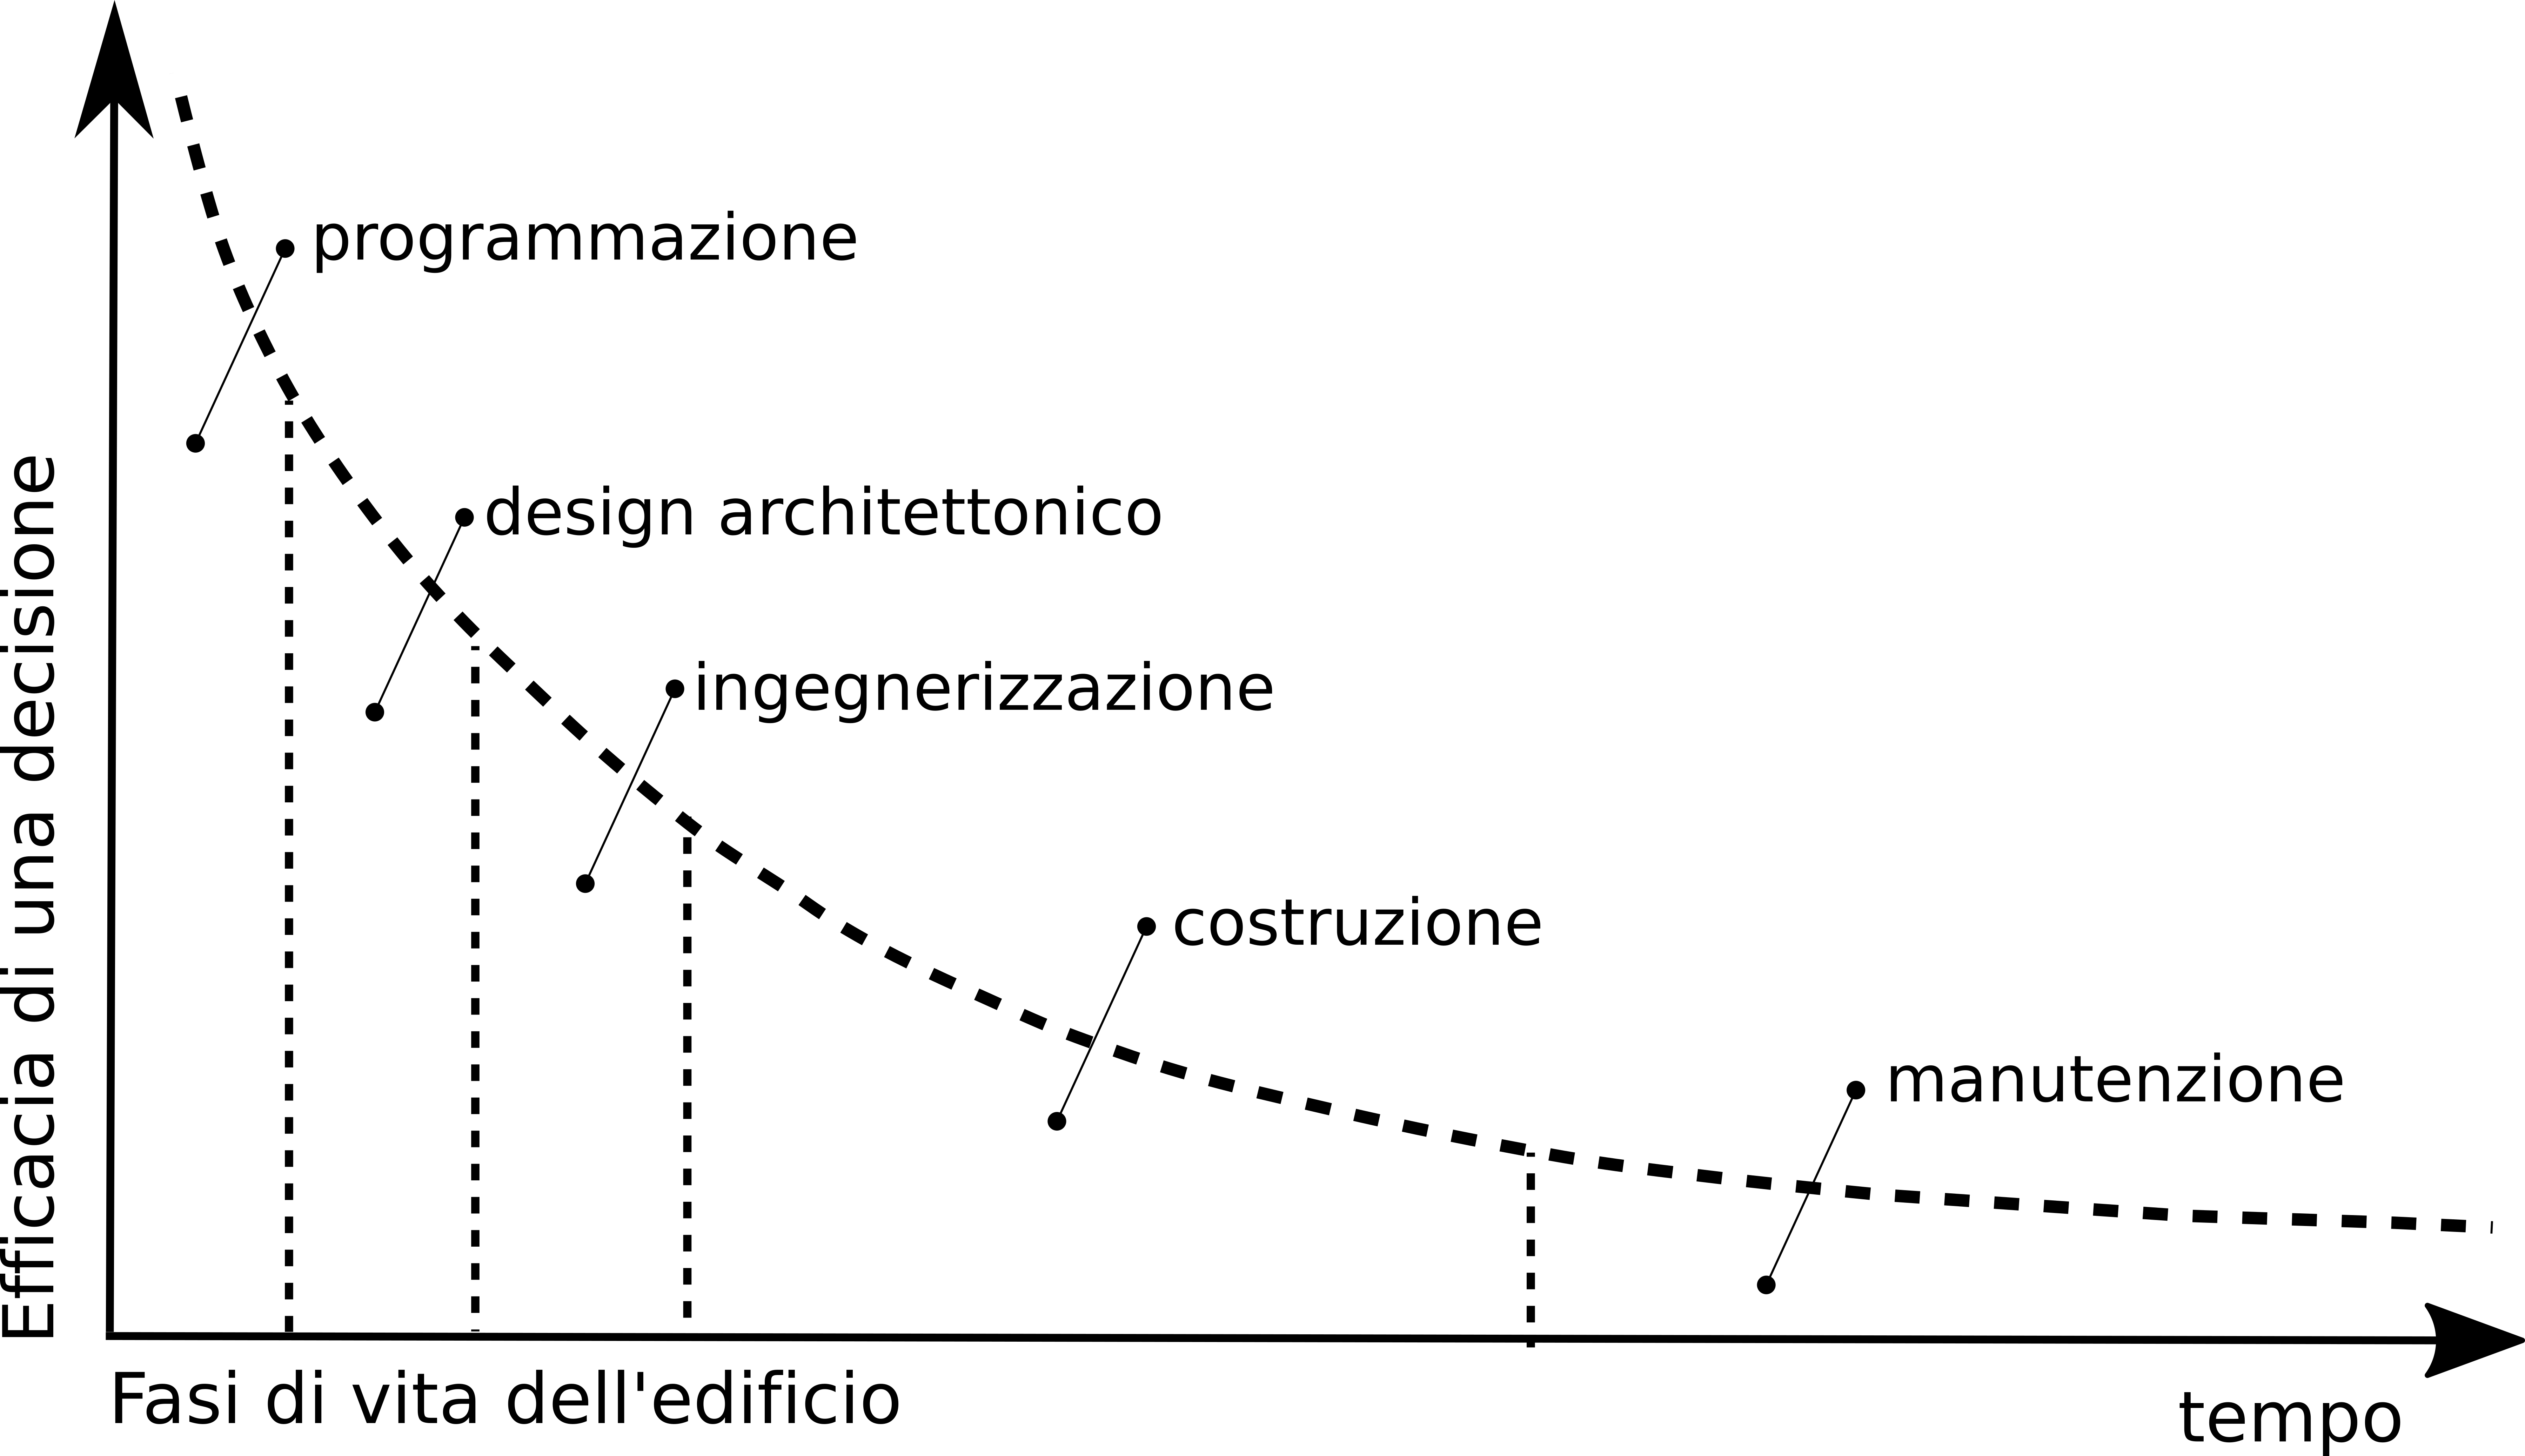
\includegraphics[width=1\textwidth,keepaspectratio]{images/lechner/efficacia-decisioni-fede}
\caption[SHORT]{Rappresentazione dell'efficacia delle decisioni nel processo edilizio.}
\label{fig:efficacia-decis-lechner}
\end{figure}


In questo senso vanno fatte alcune considerazioni semplici ma chiarificatrici. Ipotizziamo che un committente debba valutare due soluzioni progettuali per una stessa una stessa casa in uno stesso luogo:

\begin{itemize}
\item una esposta in modo coerente con il sito e con il percorso solare apparente,

\item una esposta senza prendere in considerazione i criteri del punto precedente.

\end{itemize}

È evidente come per \emph{la stessa casa} il costo della progettazione – generalmente valutato sul prezzo dell'opera – e della realizzazione risulterà sostanzialmente lo stesso. Questo aspetto potrebbe apparire poco significativo: la casa è girata in un modo piuttosto che in un altro, qualcuno potrebbe anche dire che si tratti di una questione di gusti. Ma se consideriamo che la casa esposta meglio fornisce:

\begin{itemize}
\item maggiore apporto termico invernale

\item migliore possibilità di schermatura solare estiva

\item migliori livelli di illuminamento naturale

\item condizioni meno favorevoli per la proliferazione di muffe e condense interne

\item migliori condizioni di vivibilità e quindi di benessere generale

\end{itemize}

diventa più facile, per il committente scegliere tra le due ipotesi progettuali.
%
% !TEX root = ../26_11c-all-en-amb-master-ok.tex

\chapter{CENNI DI GEOMETRIA SOLARE}
\label{chp:geometria-solare}

\section{La terra e il sole}
\label{sec:terra-sole}

Il sole fornisce \emph{energia} a tutti i pianeti del suo sistema. L'energia prodotta all'interno del nucleo – ove si raggiunge la temperatura di 14 milioni di gradi Celsius – attraverso reazioni di fusione nucleare raggiunge la terra, la riscalda e fornisce la luce naturale. 

\begin{figure}[ht]
\centering  % ordine per clip: left, lower right upper
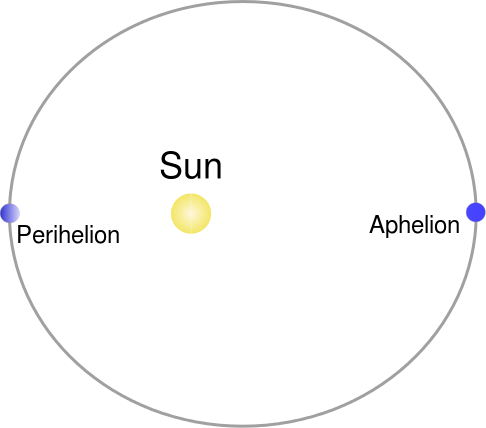
\includegraphics[width=0.4\textwidth,keepaspectratio]{images/wikipedia/Perihelion-Aphelion}
\caption[Orbita-Perielio-Afelio]{Orbita ellittica della terra attorno al sole. Si notano la posizione del sole (Sun) che non coincide con il centro dell'ellisse e le due posizioni di massima (Perihelion) e minima (Aphelion) distanza della terra dal sole. (Fonte: Wikipedia)}
\label{fig:orbita-perielio-afelio}
\end{figure}
La terra ruota attorno al sole (movimento di \emph{rivoluzione}) percorrendo un'orbita ellittica\footnote{La rivoluzione completa attorno al sole si compie in 365,25 giorni. L'eccentricità dell'ellisse è relativamente piccola e l'orbita spesso è approssimata al cerchio (vedi \fref{fig:orbita-perielio-afelio}. Il momento in cui la terra è più vicino al sole, a circa 147 milioni di km (\emph{perielio} o \emph{perihelion}) avviene il 2 di gennaio mentre il 3 luglio è il giorno in cui è più lontana, a circa 152 milioni di km (\emph{afelio} o \emph{aphelion}).} compie un giro completo che vede il sole in posizione decentrata rispetto al suo centro geometrico. Contemporaneamente la terra ruota attorno al proprio asse\footnote{In circa 24 ore compie un giro completo} (movimento di \emph{rotazione}) – che non è verticale ma inclinato di circa \ang{23,45}. Questa inclinazione è all'origine dell'alternanza delle stagioni tra i due emisferi nord e sud poiché ricevono la radiazione solare con angoli differenti: il 21 Giugno\footnote{Solstizio d'estate per l'emisfero nord e viceversa per quello sud. I raggi solari sono perpendicolari al suolo terrestre in corrispondenza del \emph{Tropico del Cancro} (latitudine di \ang{45}).} il polo Nord punta verso il sole, mentre il 21 Dicembre\footnote{Solstizio d'inverno per l'emisfero nord e viceversa per quello sud. I raggi solari sono perpendicolari\footnote{Questa situazione avviene alle ore 12 (solari) e si definisce comunemente con l'espressione: di \emph{sole allo zenit}} al suolo terrestre in corrispondenza del \emph{Tropico del Capricorno} (latitudine di~\ang{-45}).} punta verso il sole il polo Sud. In concomitanza con gli equinozi\footnote{Il 21 Marzo e 21 Settembre. In questi due giorni il centro del sole e della terra possono essere uniti idealmente tramite una linea che passa per l'equatore terrestre: ovunque, sulla terra, si avranno 12 ore di luce e 12 ore di notte, da qui il termine \emph{equinozio}, derivato dal latino che significa \emph{giorno uguale alla notte}. Va ricordato che il \emph{21esimo} giorno del mese, per solstizi ed equinozi, rappresenta una convenzione comune poiché il giorno reale, astronomico, può variare leggermente di anno in anno.} il \emph{il sole è allo zenit} alle ore 12 (solari) solo all'equatore. 

All'inclinazione dell'asse terrestre si deve quindi la definizione di un angolo (verticale) necessario per individuare la posizione del sole rispetto ad un punto qualsiasi della terra: l'angolo zenitale altrimenti definito come \emph{altitudine} solare. Si tratta cioè dell'angolo formato tra:

\begin{itemize}
\item  la retta congiungente il centro del sole ed il punto della terra in esame,
\item la proiezione di tale retta sul piano dell'orizzonte passante per il punto terrestre in questione.
\end{itemize}
 
L'effetto di questa inclinazione determina l'angolo di incidenza della radiazione solare rispetto all'atmosfera\footnote{Conseguentemente definisce anche l'angolo di incidenza al suolo terrestre.} nei diversi punti dell'orbita e di conseguenza la relativa quantità di energia che riesce ad attraversarla per raggiungere il suolo. È infatti evidente che più l'angolo di incidenza tende ad essere verticale, minore sarà la sua riflessione e quindi maggiore la percentuale di energia che potrà penetrare. Ecco perché \emph{in estate}, nonostante l'orbita terrestre ponga il nostro pianeta ad una distanza maggiore dal sole rispetto all'inverno,\footnote{Circa tre milioni di di miglia in più al 21 Giugno.} la temperatura sulla terra è maggiore: il sole è più alto sull'orizzonte, l'angolo di incidenza cresce così come la quantità di radiazione che perfora l'atmosfera e le giornate sono più lunghe.

\begin{table}[htp]
\centering
\caption{Per semplificare i calcoli e facilitare il progettista con applicazioni specifiche la tabella indica il numero di progressivo del primo giorno di ogni mese.}
\label{tab:num-primo-giorno-mese}
\begin{tabular}{@{}lclc@{}}
\toprule
\textit{mese} & \textit{num.} & \textit{mese} & \textit{num.} \\ \toprule
Gennaio       & 1             & Luglio        & 182           \\ %\midrule
Febbraio      & 32            & Agosto        & 213           \\ %\midrule
Marzo         & 60            & Settembre     & 244           \\ %\midrule
Aprile        & 91            & Ottobre       & 274           \\ %\midrule
Maggio       & 121           & Novembre      & 305           \\ %\midrule
Giugno        & 152           & Dicembre      & 335           \\ \bottomrule
\end{tabular}
\end{table}






\section{Le carte solari}
\label{sec:nota-import}

\subsection{Cosa sono}
\label{subsec:cosa-sono}


\subsection{A cosa servono}
\label{subsec:a-cosa-servono}


\subsection{Come si usano}
\label{subsec:come-si-usano}

\subsection{Carte di base per Casal Cermelli}
\label{subsec:carte-base}%
% ********************************
% -----------------------APPENDICE
% ********************************
%\appendix
\backmatter
% !TEX root = ../26_11c-all-en-amb-master-ok.tex

% v.4 copyright page - Colophon
\newpage
~\vfill
\thispagestyle{empty}
\setlength{\parindent}{0pt}
\setlength{\parskip}{\baselineskip}

\par \textsc{Comune Di Casal Cermelli (AL)}

Copyright \copyright\ \the\year\ 

\par\textsc{Published by  Comune di Casal Cermelli}
%\vfill

\par Questo Regolamento è stato compilato da Federico Morchio con \XeLaTeX\ utilizzando la classe \emph{memoir}, chapterstyle=\emph{lyhne}, oltre alcune personalizzazioni. \\
Per la composizione finale e la compilazione sono stati utilizzati:

\begin{itemize}[topsep=-3ex,itemsep=-2ex]
\item  il software \emph{TeXShop} (\url{http://pages.uoregon.edu/koch/texshop/}) su \emph{Mac OS X 10.11.6}.\\
\item Font con grazie (tondo): TeX Gyre Termes\\
\item \textsf{Font senza grazie: TeX Gyre Adventor}\\
\item \texttt{Font monospaziato: Andale Mono}
\end{itemize}

I disegni sono stati realizzati da Federico Morchio con: \\ \emph{Inkscape} (\url{https://inkscape.org/en/})

%\vfill 
\par Progetto grafico e impaginazione: Federico Morchio\\
Si ringrazia  il forum del Gruppo Utilizzatori Italiani di \TeX\ per i preziosi consigli (\url{http://www.guitex.org/home/it/forum/index})

\par \href{http://www.comune.casalcermelli.al.it/}{\texttt{www.comune.casalcermelli.al.it/}}

\par \href{http://www.oikosatelier.it}{\texttt{www.oikosatelier.it}}
\vfill

\begin{figure}[h]
\centering

\includegraphics[width=0.3\linewidth]{images/by-nc-sa-eu.jpeg}
%  \checkparity This is an \pageparity\ page.%
%\caption[][6pt]{licenza .... testo.}
\label{fig:textfig-cc-licenza}
%\zsavepos{pos:textfig}
\end{figure}
\par Quest'opera è distribuita con licenza \emph{Creative Commons Attribuzione - Non commerciale 4.0 Internazionale}.
Prima di utilizzarne il contenuto è opportuno comprendere i termini della licenza visionandoli presso il sito:\\ \href{http://creativecommons.org/licenses/by-nc/4.0/}{\texttt{creativecommons.org/licenses/by-nc/4.0/}}
\index{license}
\vfill
\par ISBN (no) \\
%\par \textbf{1}2345678910\\
\texttt{I stampa: Dicembre 2016}
% FINE COLOPHON
%

\end{document}